%Vorlage Uni, made by Oliver Wisler 25.20.2011

%set document language to german, standard font size and document size
\documentclass[ngerman, 12pt, pdftex]{scrartcl}[2006/07/30]

%encoding and input
\usepackage[ngerman]{babel} %spell correction
\usepackage[utf8]{inputenc} 
\usepackage[T1]{fontenc}
\usepackage[
	colorlinks=true,
	urlcolor=blue,
	linkcolor=green
]{hyperref}


%bugfixes
\usepackage{fixltx2e} 

%Font Symbols and Colors
\usepackage{textcomp} %more symbols
\usepackage{xcolor}

%Math
\usepackage{amsmath}
\usepackage{mathtools} %extends amsmath

%Programming
\usepackage{listingsutf8} %in utf8d
\lstset{language=Java,captionpos=b,tabsize=3,frame=lines,keywordstyle=\color{blue},commentstyle=\color{teal},stringstyle=\color{red},numbers=left,numberstyle=\tiny,numbersep=5pt,breaklines=true,showstringspaces=false,basicstyle=\footnotesize,emph={label},upquote=true} %Syntax highlighting

\usepackage{dirtree} 
\usepackage{lscape}

%Verbatim extension (with line numbers and tab-expansion)
\usepackage{moreverb} 

%Headers and Footer
\usepackage{fancyhdr}

%title
\title{CS261 Webprojekt}
\author{Frank Müller, Oliver Wisler}

\begin{document}
%declare  Header
\pagestyle{fancy}
\fancyhf{} 
\fancyhead[L]{cs261 Webprojekt} %left header
\fancyhead[C]{Dokumentation} %centered header
\fancyhead[R]{Frank Müller, Oliver Wisler}  % right header
\renewcommand{\headrulewidth}{0.1pt} 	%upper separating line
\fancyfoot[C]{\thepage} 				%centered footer, line number
%\renewcommand{\footrulewidth}{0.1pt} 	%lower separating line




%%%%%CONTENT%%%%%
%you might want to enable come features:
%\maketitle
\tableofcontents
\newpage


\section{Installation}

Für die Installation müssen folgende Schritte durchlaufen werden:
\subsection{Installation der Dateien}
    Bitte kopieren Sie alle Dateien in das gewünschte Stammverzeichnis.
    Ihr Webserver muss PHP und MySQL unterstützen, um diese Webseite anbieten zu können. Unter Umständen müssen Sie die Pfade der Datei \verb+./.htaccess+ an Ihre Serverinstallation anpassen.
\subsection{Setzen der Konstanten}
    Setzten Sie alle wichtigen Konstanten in \verb+./config.php+.
    Die Verwendung und Bedeutung der Konstanten wird in der Datei erklärt.
    Achten Sie darauf, dass die Konstante \verb+INSTALL+ auf den Wert 1 gesetzt wird.
\subsection{Installation der Datenbank} % (fold)
\label{sub:Installation der Datenbank}
    Stellen Sie sicher, dass die in  \verb+./config.php+ angegebene Datenbank existiert.
    Führen Sie die Datei  \verb+./db_setup.php+ mit PHP aus. Alternativ können Sie auch 
    die url  \url{http://www.IhreWebsite.ch/Pfad_zu_db_setup.php/db_setup.php} aufrufen.
% subsection Installation der Datenbank (end)
\subsection{Einrichten} % (fold)
\label{sub:Einrichten}
	\paragraph{Root-Benutzer}
		Es wird ein Hauptbenutzer angelegt. Sie müssen für diesen Benutzer ein Passwort festlegen. 
		Dies geschieht mit dem Aufruf von \url{http://www.IhreWebsite.ch/Pfad_zu_setRootPass.php/setRootPass.php?passwd=IhrPasswort}.
		Ersetzen Sie \verb+IhrPasswort+ mit einem sicheren Passwort.
	\paragraph{Installation abschliessen}
		Nun können Sie die Konstante \verb+INSTALL+ auf 0 setzen. Die Installation ist somit abgeschlossen.
		\paragraph{Bemerkung}
    Das \verb+./uploads/+ Verzeichnis muss für php beschreibbar sein. Setzen Sie wenn nötig die erforderlichen Rechte
    (zum Beispiel mit \verb+chgrp http ./uploads+). 
  


% subsection Einrichten (end)


% section  (end)

\section{Umsetzung}
\subsection{Funktionsumfang}
	\subsubsection{Geplant}
		\begin{enumerate}
		\item Verschiedene Benutzer mit verschiedenen Aufgabenbereichen
		\item Aufträge können von allen Benutzern bearbeitet werden
		\item Jeder Auftrag soll einen Verlauf haben
		\item Zuordnen von Aufträgen an Benutzern, weiterreichen von Aufträgen
		\item Ein Auftrag durchläuft verschiedene Stufen
		\end{enumerate}
	\subsubsection{Umsetzung}
		Hier jeweils ein kurzer Kommentar zur Umsetzung der verschiedenen Zielsetzungen
		\begin{enumerate}
				\item Wurde umgesetzt mit 3 Benutzergruppen (Verwaltung, Lagerist, Arbeiter)
				\item Alle Aufträge sind von zuständigen Benutzern veränderbar
				\item Der Verlauf wurde als XML-Datei realisiert
				\item Aufträge können zugeordnet und weitergereicht werden, jedoch fehlt eine Art Übersicht über die Zuordnungen
				\item Der Auftrag durchläuft verschiedene Stufen (Erfassung, Abarbeiten, Abrechnen, Archiv)
		\end{enumerate}

% subsection  (end)
\subsection{Aufbau}
	\subsubsection{Dateisystem}
Unsere Ordnerstruktur ist so gestaltet, dass alle Dateien nach Funktion aufgeteilt werden.
Das Zusammensetzen der dargestellten Seite wird dabei von der Datei \verb+index.php+ übernommen. 
Dass heisst, fast alle Funktionalitäten unserer Seite sind über \verb+index.php+ erreichbar.
Javascript Dateien werden nur nach Bedarf geladen.
\dirtree{%
 .1 /. 
 .2 installfiles\DTcomment{Installationsdateien}. 
 .2 templates\DTcomment{Vorlagen für die Seiten}. 
 .2 css\DTcomment{CSS Dateien}. 
 .2 js\DTcomment{Javascript Dateien}. 
 .2 handlers\DTcomment{Ajax Handler / REST-Interface}. 
 .2 img\DTcomment{Bilder}. 
 .2 uploads\DTcomment{Hochgeladene Dateien}. 
 .2 doc\DTcomment{Dokumentation}. 
}
		
	\subsubsection{Seitenaufbau}
	Hier der exemplarische Aufbau unserer \verb+index.php+ Datei. 
	Der jeweilige Seiteninhalt wird dynamisch als \verb+<article></article>+ eingebunden.
	Javascript Dateien werden spezifisch für jede Seite eingebunden.
	
	\lstset{language=html}
\begin{lstlisting}
<html>
	<head>
		<!-- Hier sind alle CSS Dateien eingebunden -->
	</head>
	<body>
		<div id="content">
			<header>
				<!-- Hier ist das Menu -->
			</header>
			<!-- Benachrichtigungsfeld -->
			
			<article>
				<!-- hier ist der verlangte Seiteninhalt -->
			</article>
					
					
		</div>
		<!-- Hier sind alle Javascript Dateien eingebunden -->
	</body>
</html>
	\end{lstlisting}
	
	\subsubsection{Benutzerinteraktionen}
	Unsere Seite setzt sehr viel Javascript für die Benutzerinteraktionen ein. 
	Rund 7\% unseres Codes ist Javascript. Wo möglich wurden viele Interaktionen mittels Ajax gelöst.
	Jedoch ist ein neu laden der Seite manchmal unumgänglich. 
	
	
	
	\subsubsection{Benutzerführung}
	Folgende Graphik zeigt unsere Benutzerführung.
	\begin{figure}[h!]
 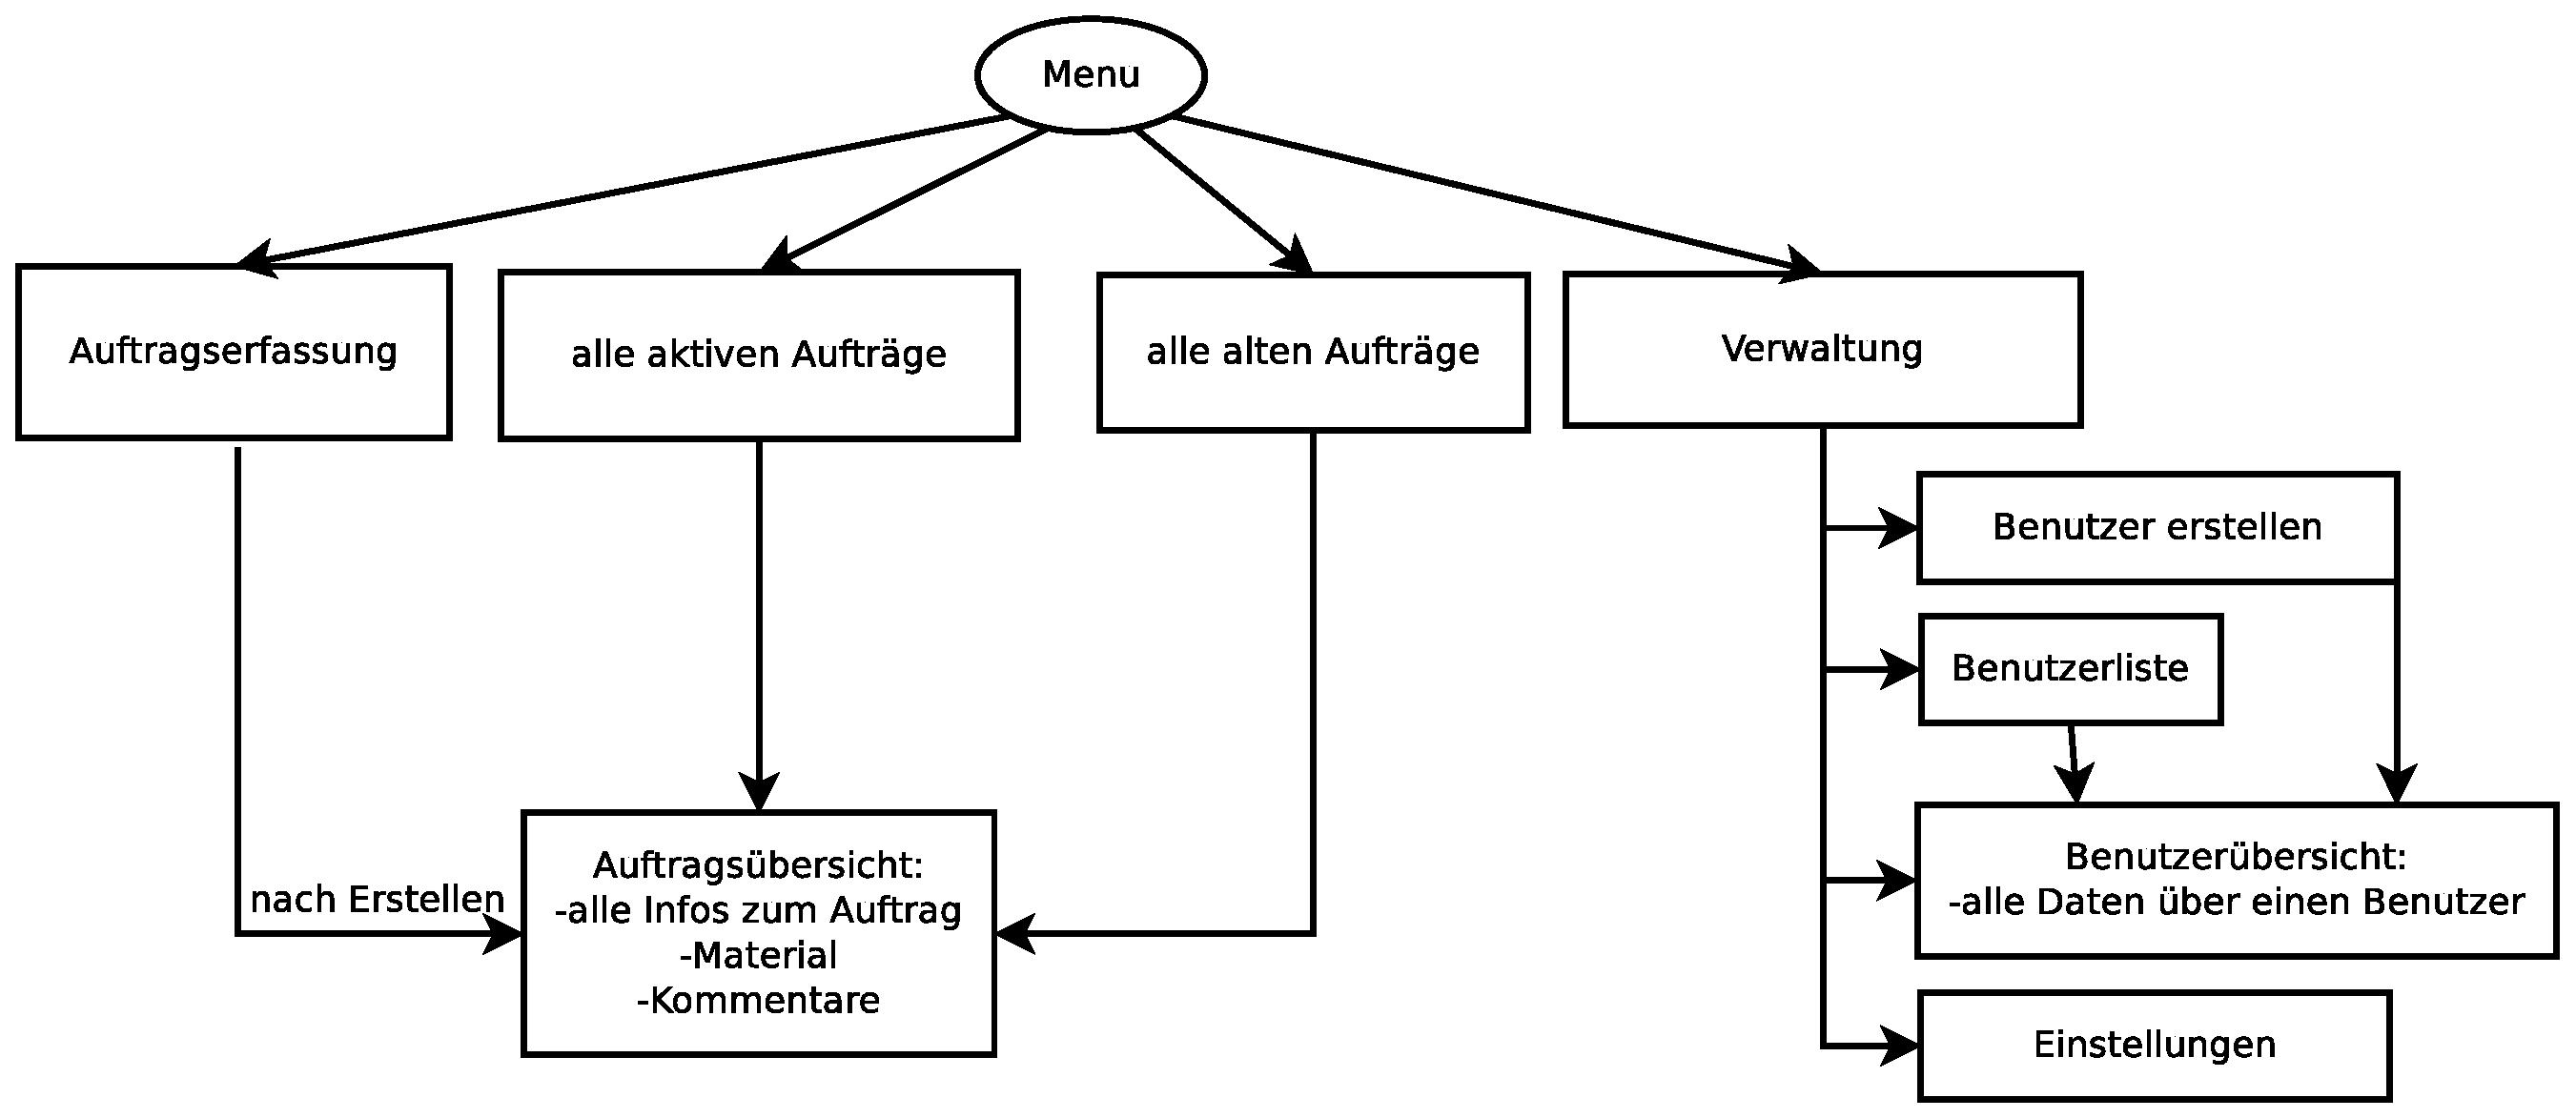
\includegraphics[width=\textwidth]{navigation.eps}
\end{figure}

% subsection  (end)
\subsection{Datenbank}
Auf folgenden Graphiken ist unser Datenbankschema dargestellt. 
Beim Verlauf wollten wir ursprünglich noch Benachrichtigungen für Benutzer zur
Verfügung stellen. Aus Zeitgründen haben dies jedoch nicht mehr implementiert.
Auch die Verknüpfung des Verlaufes mit den einzelnen Datenbankeinträgen ist zwar laut Schema
vorgesehen, jedoch nicht implementiert. Wir haben absichtlich keine Trigger / Stored Procedures verwendet, da diese
von den meisten Hostern nicht unterstützt werden.
\begin{figure}[hbt]
	\centering
	\includegraphics[scale=0.9]{./db_pdfs/history.pdf}
	\caption{Tabellen welche für die Benachrichtigungen (Updates) und Rückverfolgbarkeit zuständig sind.}
\end{figure}


\begin{landscape}
\begin{figure}[p]
	\centering
	\includegraphics[scale=0.6]{./db_pdfs/everything.pdf}
	\caption{Das gesamte Datebankschema}
\end{figure}
\end{landscape}

\begin{figure}[h!p]
	\centering
	\includegraphics[scale=1]{./db_pdfs/jobs.pdf}
	\caption{Alle Tabellen in denen Informationen betreffend eines Auftrages sind.}
\end{figure}



\newpage

% subsection  (end)
% section  (end)
\subsection{Verwendete Komponenten und Bibliotheken} % (fold)
\begin{itemize}
\item jQuery \url{http://jquery.com/} (Javascript-Bibliothek)
\item Iconic \url{https://github.com/somerandomdude/Iconic}(Icons)
\item SuperBox \url{http://pierrebertet.net/projects/jquery_superbox/}(Javascript Overlay)
\item tinyMCE \url{www.tinymce.com/}(Texteditor)
\item AjaxFileUploader \url{https://github.com/jfeldstein/jQuery.AjaxFileUpload.js}(Asynchron Dateien hochladen)
\end{itemize}



\section{Benutzeroberfläche}
\subsection{Verwaltung}
In der Verwaltung eingeteilte User haben das Privileg neue Benutzer hinzuzufügen und Passwörter anderer User zurückzusetzen.
% subsection  (end)
\subsection{Lagerist}
Der Lagerist kann ihm zugewiesene Aufträge editieren, Materialien editieren, hinzufügen und den Auftrag einer andern Person zuweisen.

% subsection  (end)

\subsection{Arbeiter}
Der Arbeiter kann ihm zugewiesene Aufträge editieren und an andere Personen zuweisen.

% subsection  (end)
% section  (end)

\section{Fazit}
\subsection{Einschränkungen}
\begin{itemize}
\item Ein Nutzer kann nur Aufträge sehen/bearbeiten, die ihm zugewiesen sind(Es handelt sich hier um eine gewollte Einschränkung).
\item Gewisse Interaktionen sind nicht Asynchron ausgeführt
\item Benutzerverwaltung ist rudimentär
\end{itemize}

% subsection  (end)

\subsection{Problemstellen}
\begin{itemize}
\item Sind die Zugriffsrechte im Dateisystem so gesetzt , dass \verb+./uploads/+ nicht durch php mit Dateien gefüllt werden kann, so kann dies zu unerwünschtem Verhalten führen.
\item Da php die hochgeladenen Dateien im \verb+/tmp+ Verzeichnis zwischenspeichert, kann dies zu Problemen führen, wenn \verb+/tmp+ als tmpfs gemounted ist und die Summe über die Grössen aller gleichzeitig hochgeladenen Dateien zu gross ist.
\item Die Website funktioniert nicht korrekt mit alten Internet Explorer Versionen. Wir bitten IE Nutzer deshalb einen Browser mit HTML5-Unterstützung zu benutzen.

\end{itemize}
% subsection  (end)
\subsection{Lessons learned}
\begin{itemize}
\item Asynchronder Dateiupload geht nicht nativ mit jQuery.
\item Auswerten von grösseren Formularen ist sehr repetitive Arbeit. Diesbezüglich war das von uns gewählte Projekt suboptimal.
\item Ajax benötigt klare Abmachungen der Schnittstellen und ist sehr zeitaufwendig
\item Browser $\neq$ Browser
\item Keine langen Unterbrüche machen (Einarbeitungszeit)
\end{itemize}

% subsection  (end)

% section  (end)
\end{document}]
